\chapter{Превращение флагов}
\label{ch:draughts-moves}

\begin{marginfigure}[-2em]
{%
\setlength{\fboxsep}{0pt}%
\setlength{\fboxrule}{1pt}%
\fcolorbox{gray}{gray}{
\includegraphics{./commons/Flag_of_Republika_Srpska.png}}%
}%
%
\includegraphics{./commons/Flag_of_Republika_Srpska.png}
%\fcolorbox{white}{gray}{
\includegraphics{./commons/Flag_of_Republika_Srpska.png}}

\caption{Флаг Сербии. Какие ещё два флага можно получить, слегка меняя оттенки 
    и сдвигая горизонтальные полоски вверх или вниз? 
    См. ответ~\ref{answer:Tricolor-flags} на с.~\pageref{answer:Tricolor-flags}.}
\label{fig:Srpska}
\end{marginfigure}

\newthought{В нашей задаче} будет дана стопка горизонтальных полосок разных цветов, 
из которых можно составить флаги государств. Сначала в игре показывают такие флаги и сообщают названия государств.
Игроку нужно расположить горизонтальные полоски так, чтобы они составили какой-либо известный флаг. 

Сузим задачу, ограничимся только трёхцветными флагами, как у России 
или Сербии (рис.~\ref{fig:Srpska}).
А по цветовой гамме выберем только флаги с белыми, синими или красными цветами.

\newthought{Сколько} таких флагов? И у каких государств? Ответы на эти вопросы 
можно найти с помощью Викиданных %\marginnote{
% }. 
На Викиданных представлены \href{http://bit.ly/2OgIdWo}{328 государственных флага}\footnote[][-3cm]{
    SPARQL-запрос к Викиданным для получения списка государственных флагов: \url{http://bit.ly/2OgIdWo}
}, 
причём с тремя горизонтальными полосками по версии Викиданных 
существует \href{http://bit.ly/2Q96ET1}{101 флаг}\footnote[][-2.8cm]{
    Список горизонтальных триколоров по Викиданным
    \url{http://bit.ly/2Q96ET1}
}. 
Горизонтальных триколоров с красным, белым и синим цветом 
имеют всего \href{http://bit.ly/2xDTXsI}{19 государств}\footnote[][-2.0cm]{
    Только синие, белые и/или красные цвета у триколоров 
    \url{http://bit.ly/2xDTXsI}
    \bigskip 
}.

\marginnote[-0.5cm]{
    О языке SPARQL и объектах Викиданных читайте в курсе Викиверситета ``Программирование Викиданных'' 
    \href{https://ru.wikiversity.org/wiki/\%D0\%9F\%D1\%80\%D0\%BE\%D0\%B3\%D1\%80\%D0\%B0\%D0\%BC\%D0\%BC\%D0\%B8\%D1\%80\%D0\%BE\%D0\%B2\%D0\%B0\%D0\%BD\%D0\%B8\%D0\%B5_\%D0\%92\%D0\%B8\%D0\%BA\%D0\%B8\%D0\%B4\%D0\%B0\%D0\%BD\%D0\%BD\%D1\%8B\%D1\%85}{https://ru.wikiversity.org}.
}

\begin{mdfstyle}[nobreak=true,frametitle=На каком языке компьютеры читают Википедию?]
\sloppy 
    \index{Викиданные}Викиданные -- это компьютерная система, включающая базу данных, интерфейс для редактирования и язык запросов SPARQL для поиска в базе. Как и Википедию, Викиданные может редактировать каждый. Программисты любят Викиданные, потому что это та же Википедия, но в машиночитаемом виде, то есть язык Викиданных понимают и роботы, и компьютерные программы.
% \marginnote{Hello}
\end{mdfstyle}

\begin{marginfigure}[-4cm]
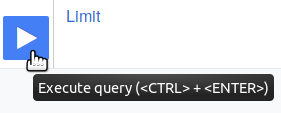
\includegraphics{./wikidata/play_blue_button_wikidata.png}
%\fcolorbox{white}{gray}{
\includegraphics{./commons/Flag_of_Republika_Srpska.png}}

    \caption[Кнопка Play на странице выполнения SPARQL-запросов к Викиданным]{Кнопка 
    Play на странице ``Wikidata Query'' для запуска SPARQl-скриптов.
    Вместо клика по кнопке можно нажать комбинацию клавиш <Ctrl>+<Enter>.}
  \label{fig:blue:button}
\end{marginfigure}

\begin{marginfigure}[-0cm]
  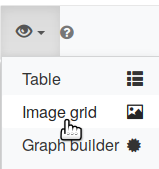
\includegraphics[width=0.5\columnwidth]{./wikidata/image_grid_select.png}
%  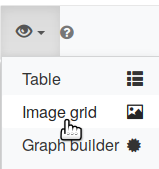
\includegraphics{./wikidata/image_grid_select.png}
  \caption[Выбор представления результатов SPARQL-запроса в виде мозаики 
    иллюстраций.]{Выбор представления результатов SPARQL-запроса 
    в виде мозаики иллюстраций. Нажмите на значок глАза, затем выберите 
    пункт ``Image grid'' в выпадающем меню.
}
  \label{fig:wd:grid:select}
\end{marginfigure}


\newthought{Эти короткие ссылки}, например, \url{http://bit.ly/2OgIdWo}, 
приведут вас на страницу ``Wikidata Query'', 
то есть на страницу запросов к базе Викиданных на языке SPARQL. 
Чтобы запустить запрос, нажмите на кнопку Play (рис.~\ref{fig:blue:button}). 
Для превращения скучного списка названий флагов в мозаику флагов, 
щёлкните по значку глАза, затем выберите пункт выпадающего меню 
``Image grid'' (рис.~\ref{fig:wd:grid:select}).% \sidenote[][-3.0cm]{This sidenote is 1 centimeter higher than it normally would be and uses its original sidenote number.}





\begin{mdframed}[nobreak=true]
\sloppy % Text doesn't wrap correctly inside an mdframed frame (in tufte-book), see https://tex.stackexchange.com/a/153877/99685
    \index{короткие ссылки@Короткая ссылка}Короткие ссылки создаются специальными сайтами, которые берут длиннющую 
    гиперссылку и превращают её в коротенький набор букв и цифр. Это удобно, 
    если вы хотите оставить место в сообщении для своего текста и 
    не тратить драгоценные знакоместа на кашу из символов в URL.  
    Таких сервисов по сокращению URL много, bit.ly -- это один из них. 
    А почему сервис bitly называется bitly? Потому что ссылки становятся "a little BIT smaller", то есть "чуть-чуть покороче". 
    И потому что ``бит'' (англ. bit) -- это крошечное количество данных. 
    % Source: Why is it called Bitly? Annelise Schoups, 2016. URL: https://www.rewindandcapture.com/why-is-bitly-called-bitly/
\end{mdframed}

\begin{marginfigure}
{%
\setlength{\fboxsep}{0pt}%
\setlength{\fboxrule}{1pt}%
%\fcolorbox{gray}{gray}{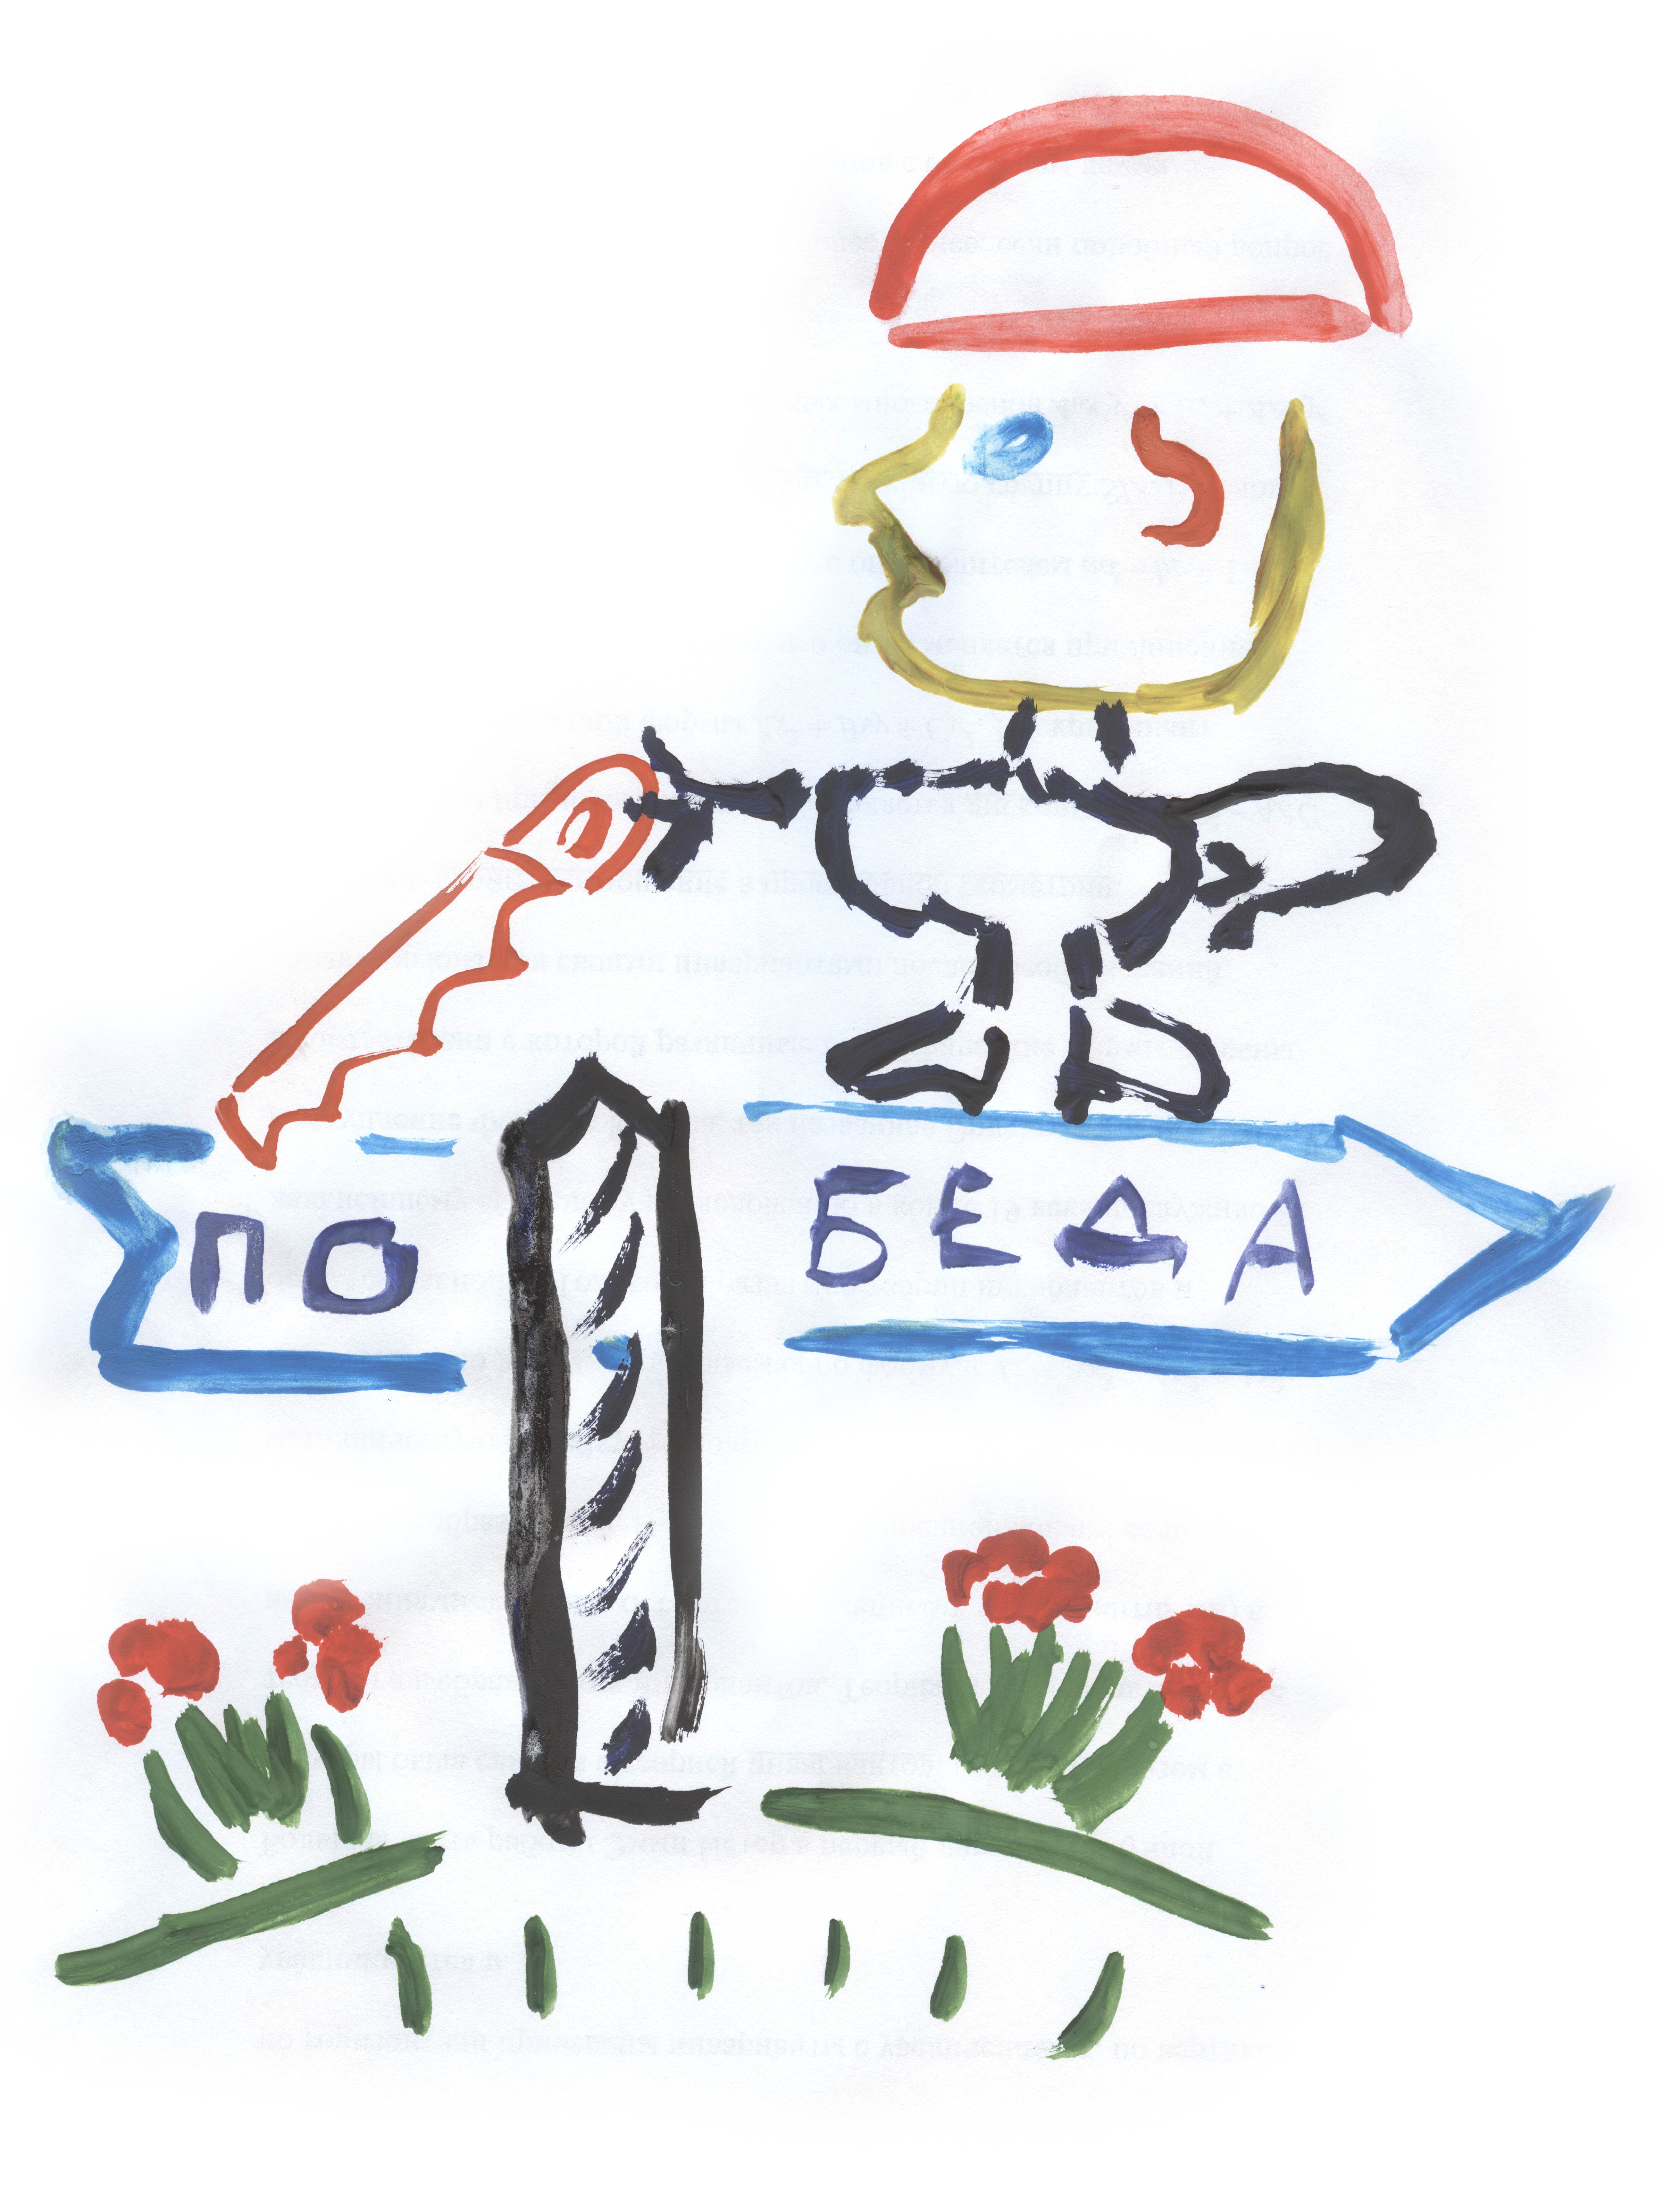
\includegraphics{./graphics/sketch/short_link_knauff_pobeda_v3.jpg}}%
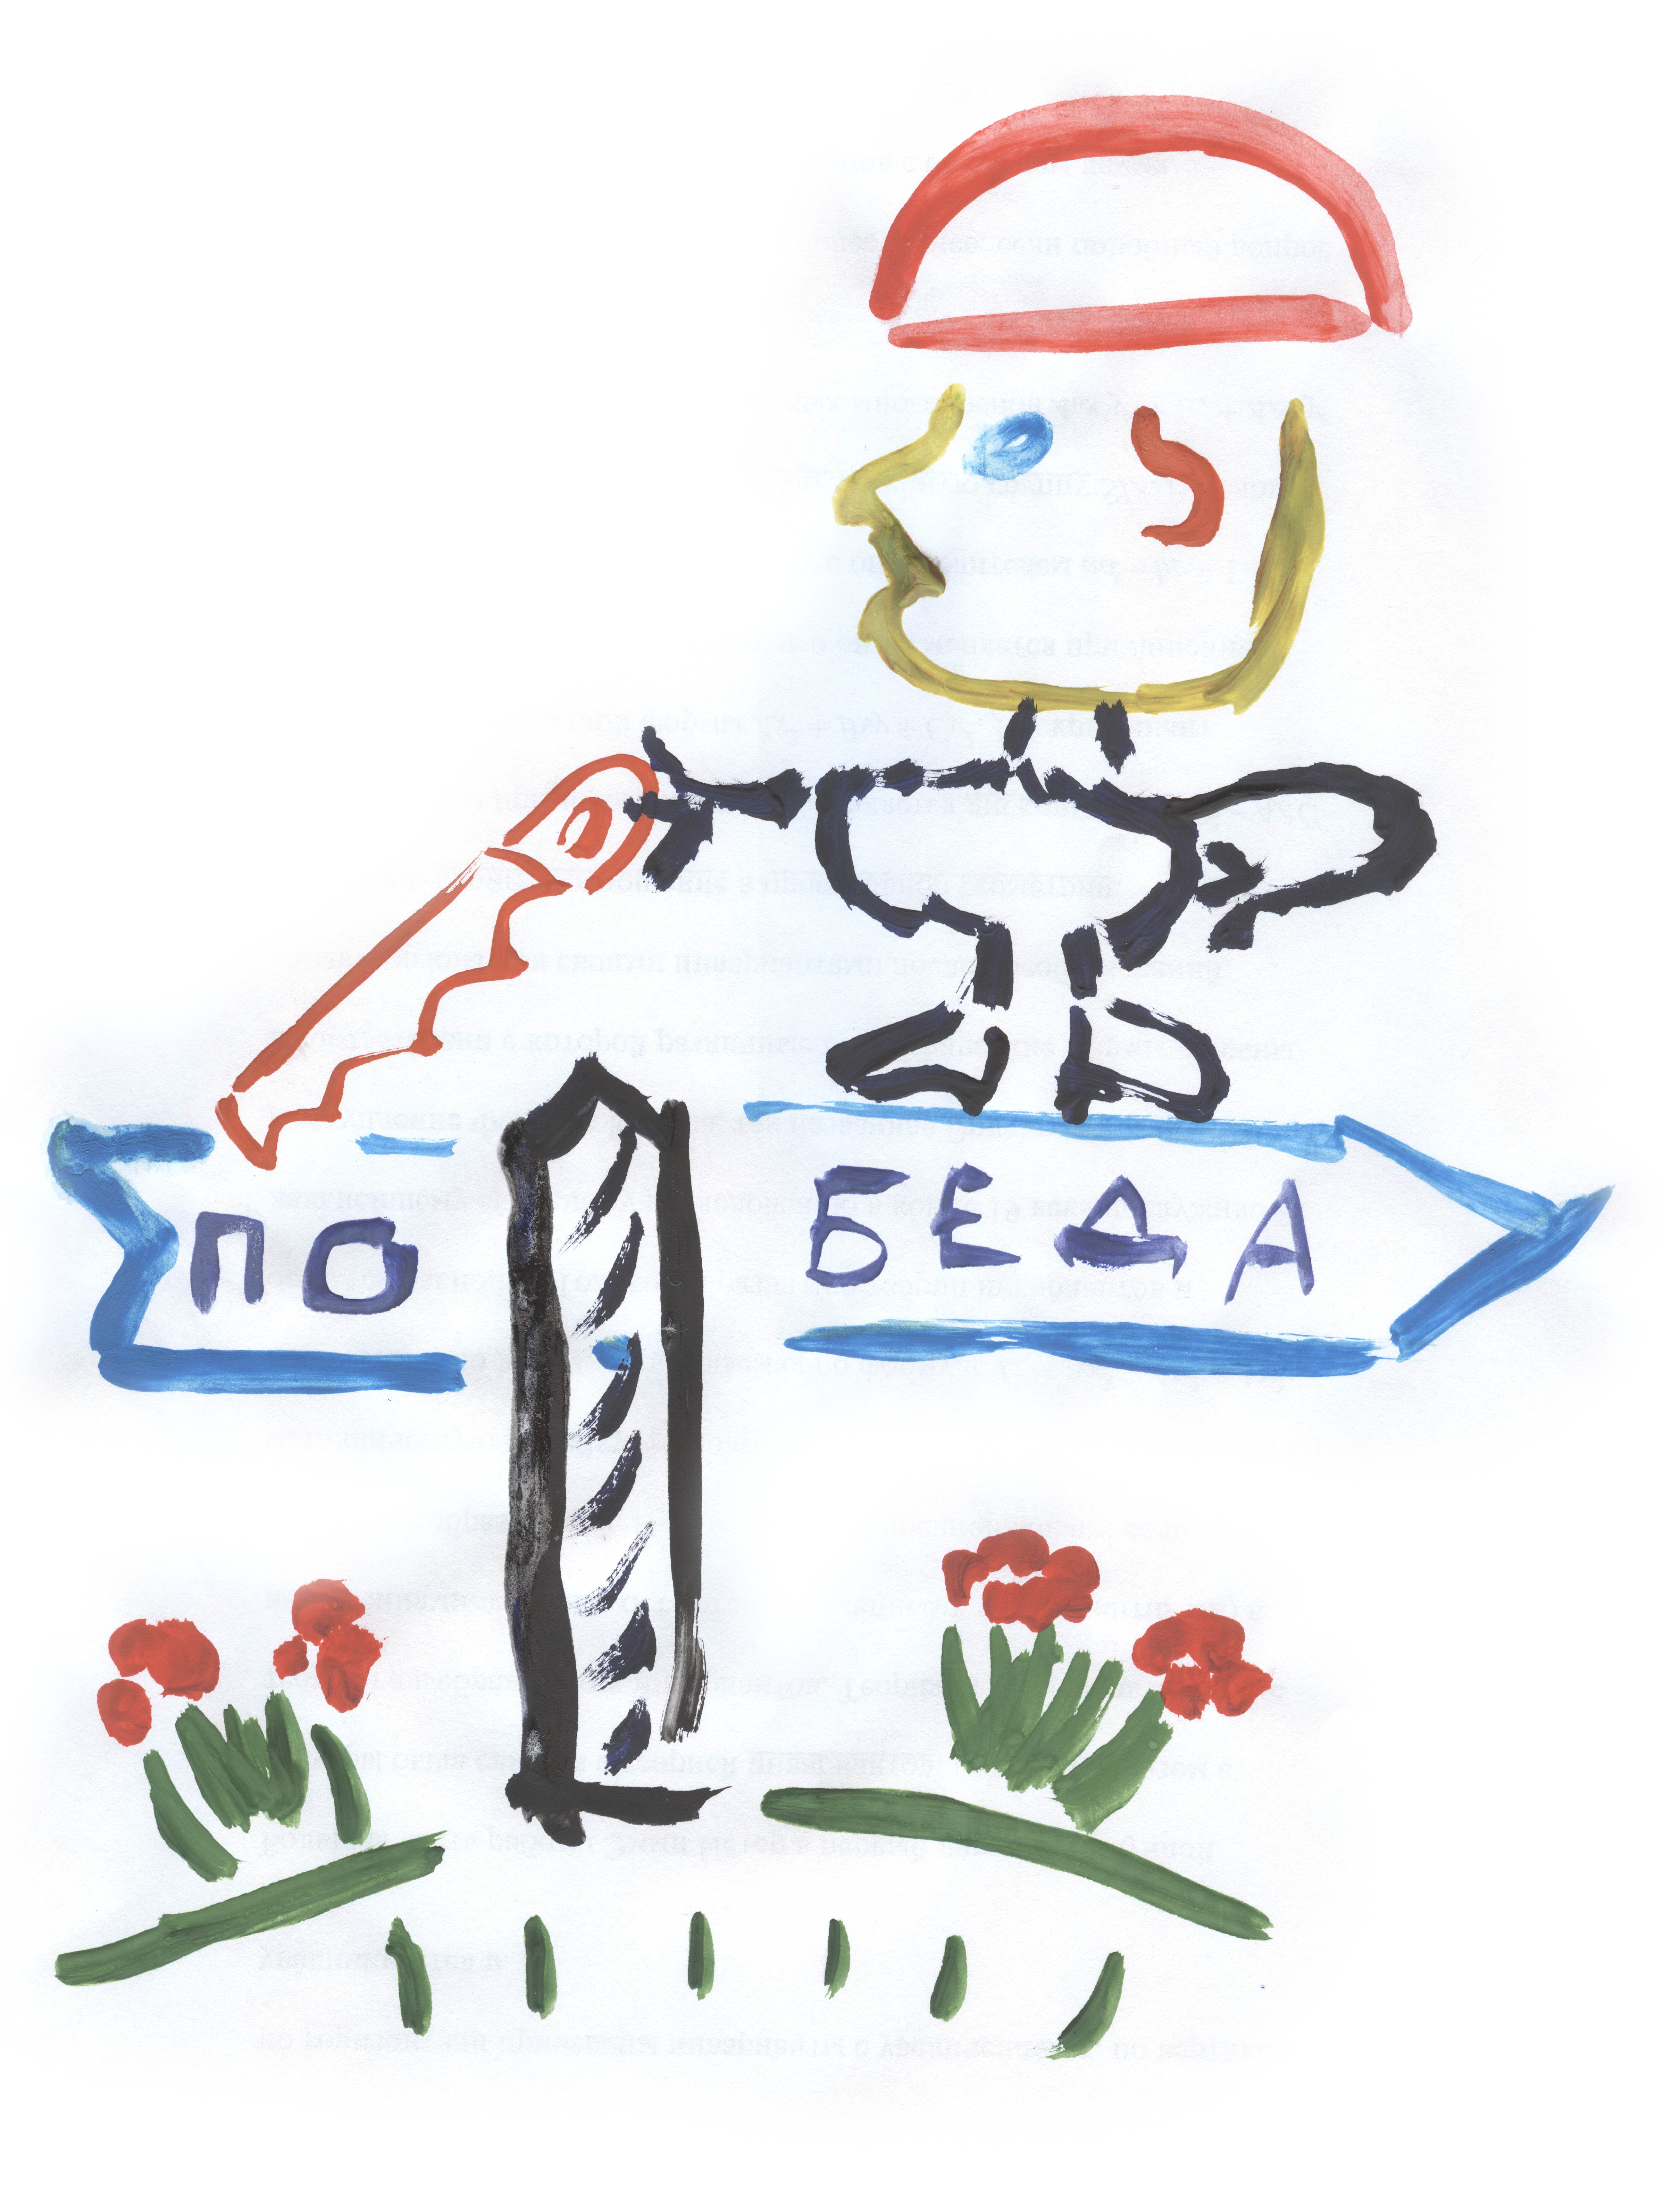
\includegraphics{./graphics/sketch/short_link_knauff_pobeda_v3.jpg}
}%
%
\includegraphics{./commons/Flag_of_Republika_Srpska.png}
%\fcolorbox{white}{gray}{
\includegraphics{./commons/Flag_of_Republika_Srpska.png}}

\caption{Есть разные подходы и алгоритмы для укорачивания ссылок и имён. В~каком 
    мультфильме название корабля в начале плавания стало короче задуманного и почему?
    См. ответ~\ref{answer:Pobeda-beda} на с.~\pageref{answer:Pobeda-beda}.}
\label{fig:Pobeda-beda}
\end{marginfigure}

Задача: сколько ссылок можно закодировать, 
        если ссылка содержит ровно 7 буквенно-цифровых символов,
        каждый символ может быть буквой английского алфавита 
        или цифрой от 0 до 9? Ответ на странице ... todo.

Temp indexkey example: А вот и \index{Интерфейс пользователя!ListView / Выбор из списка}...
